$g = \dfrac{\sqrt{1+\dot x^2}}{x}$


Euler–Lagrange equation:
$$\dfrac{\partial g}{\partial x} - \dfrac{d}{dt}\dfrac{\partial g}{\partial \dot x} = 0$$
$g$ is a function of $x$ and $\dot x$ so:
$$g - \dot{x}g_{\dot x} = C$$
$C$ is constant.
$$g_{\dot{x}} = \dfrac{\dot x}{x\sqrt{1+\dot x^2}}$$
$$\dfrac{1}{x\sqrt{1+\dot x^2}}=C$$
Above equation solved in MATLAB(Q5\_f.m) with boundary condition $x(0) = 0$.
$$x(t) = \pm \dfrac{\sqrt{-c\,t\,{\left(c\,t+2\right)}}}{c}$$
Final time: 
$(t_f - 9)^2 + x^2(t_f) = 9$


We can change $\theta_{t}$ to:
$$\theta(t) = \pm \sqrt{9 - (t_f-9)^2}$$
$$\left.(g + (\dot{\theta}-\dot{x})g_{\dot{x}})\right\vert_{t = t_f}  = 0 \to (9-t_f)^2(\dot x_{tf}^2-1) = 9$$

$$\dot x =\pm \frac{ct-1}{\,
	\sqrt{-c\,t\,{\left(c\,t-2\right)}}}$$
\begin{align*}
	(t_f - 9)^2 + \dfrac{{-t_f\,{\left(c\,t_f+2\right)}}}{c} &= 9\\	
	(9-t_f)^2(\frac{(ct_f-1)^2}{\,
		{-c\,t_f\,{\left(c\,t_f-2\right)}}}) & = 9
\end{align*}
There is two equation and two unknowns.
Above equation solved in MATLAB(Q5\_f.m).



$c = -0.1679, \quad t_f = 11.8267$

\begin{figure}[H]
	\caption{Answer Figure}
	\centering
	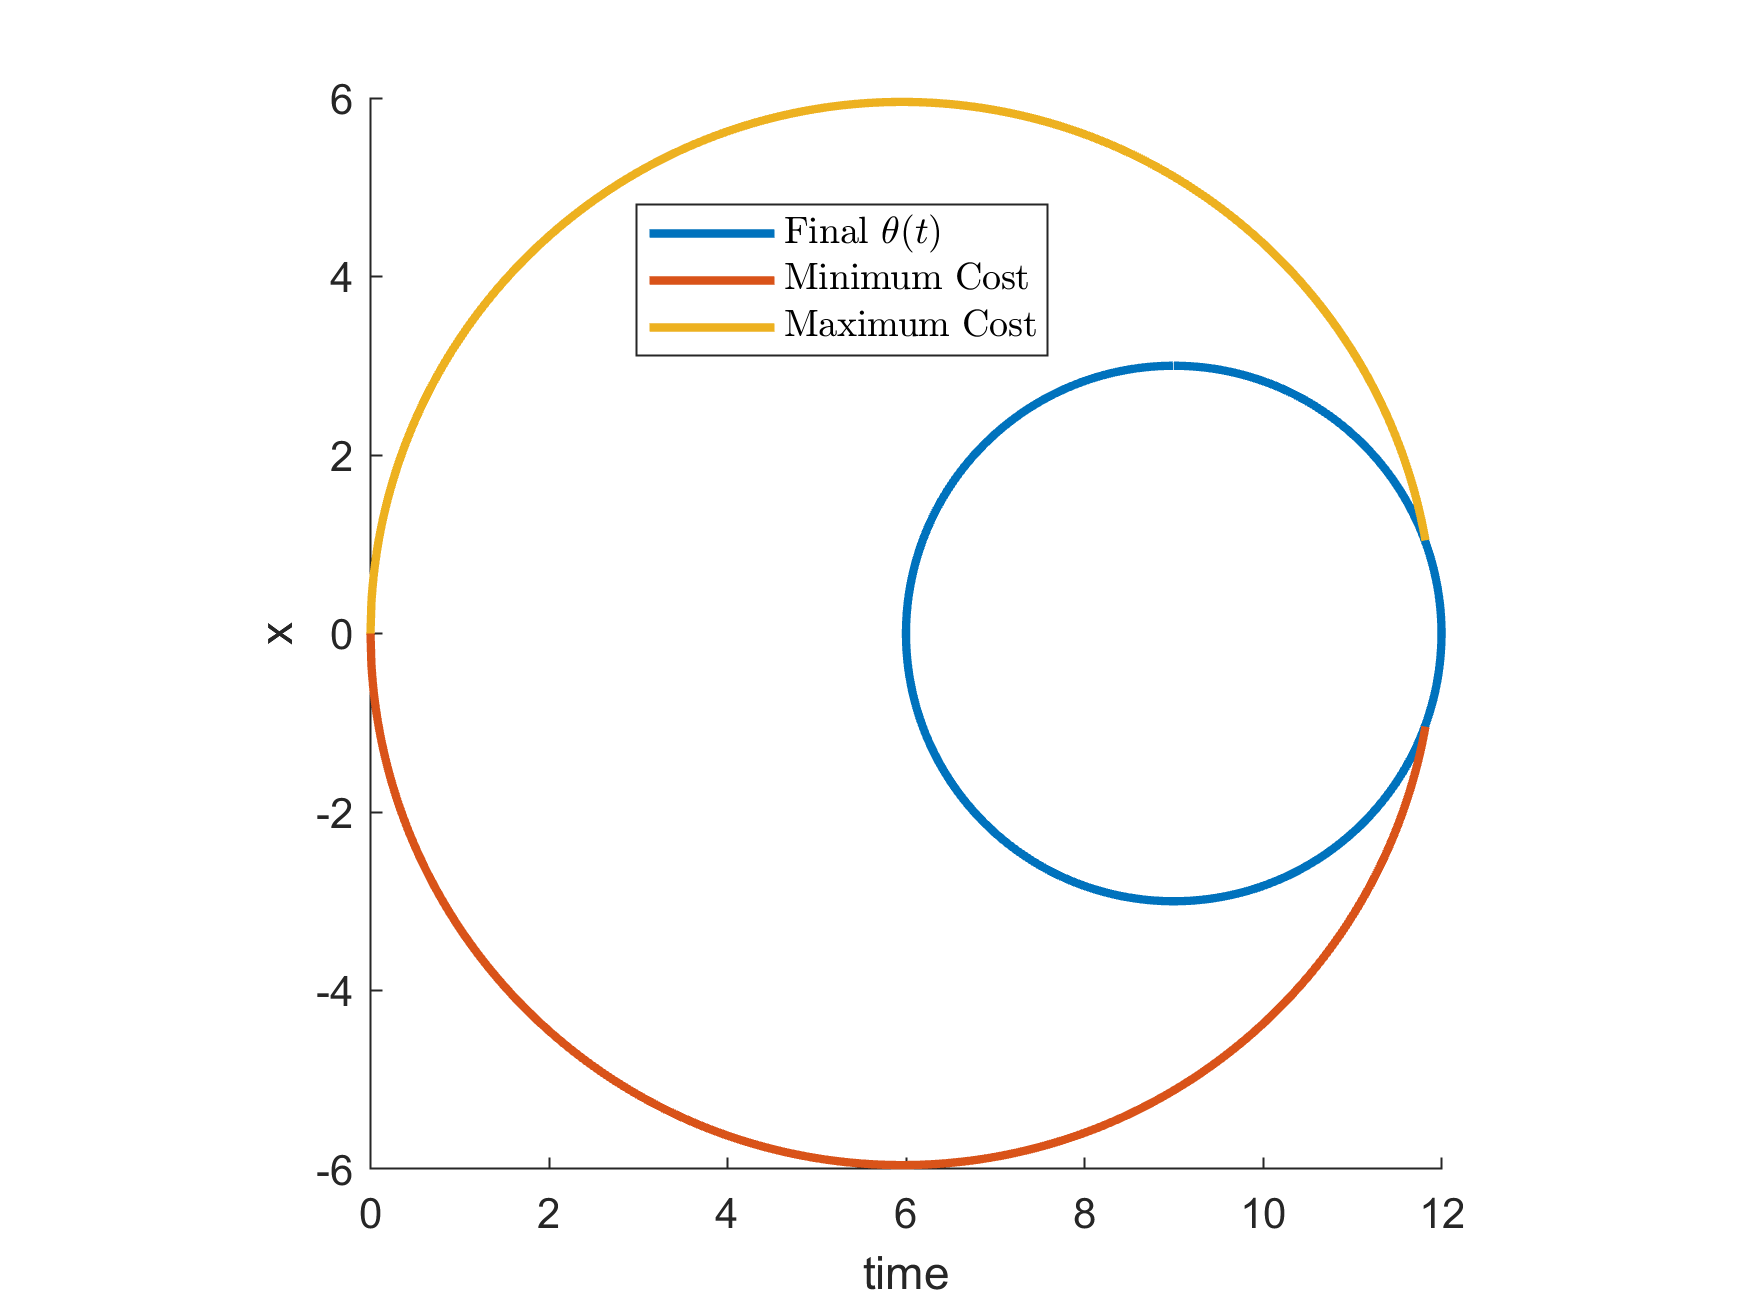
\includegraphics[width=12cm]{Q5/figures/Figure5fFix.png}
\end{figure}
